% !Mode:: "TeX:UTF-8"
% !TEX program  = xelatex
% !BIB program  = biber
\documentclass{ctexbeamer}
  % !Mode:: "TeX:UTF-8"
% !TEX program  = xelatex
% 使用的宏包
\usepackage{zhlipsum,lipsum}
\usepackage{booktabs}
\usepackage[style=gb7714-2015]{biblatex}
  \addbibresource{references.bib}

% logo 设置
\usepackage{textpos}
  \addtobeamertemplate{frametitle}{}{%
    \begin{textblock*}{100mm}(.85\textwidth,-0.7cm)
      \includegraphics[height=0.5cm]{figures/logo/SUSTech-zh.pdf}
    \end{textblock*}
  }
\mode<presentation>{
  \setbeamercovered{transparent}}
% 字体与主题
\setbeamertemplate{navigation symbols}{}
\usetheme{CambridgeUS} % or other themes, see http://www.hartwork.org/beamer-theme-matrix/
\usefonttheme{professionalfonts}
\usefonttheme[onlymath]{serif}
% 标题页
\AtBeginDocument{
  \begin{frame}
    \titlepage
    \vfill\hfill
    \inserttitlegraphic{\includegraphics[height=0.5cm]{figures/logo/SUSTech-zh.pdf}}
  \end{frame}
  \addtocounter{framenumber}{-1}
}
% 目录
\AtBeginSection[]{
  \begin{frame}<beamer> % [shrink]
    \frametitle{Outline}
    \tableofcontents[currentsection]
  \end{frame}
}
% 颜色设置
\mode<presentation>
  \definecolor{tbg}{rgb}{0.0,0.39,0.62}
  \definecolor{tfg}{RGB}{255,227,189}
  \definecolor{ftbg}{RGB}{220,224,224}
  \definecolor{colorA}{RGB}{60, 60, 40}
  % or structure
  \setbeamercolor*{structure}{bg=tfg, fg=tbg}
  % or subtitle
  \setbeamercolor*{frametitle}{use=structure, bg=ftbg, fg=structure.fg}
  % radient top color
  \setbeamercolor*{palette primary}{use=structure,  fg=structure.bg, bg=structure.fg}
  \setbeamercolor*{palette secondary}{use=structure,fg=structure.bg, bg=structure.fg!75!black}
  \setbeamercolor*{palette tertiary}{use=structure,fg=structure.bg, bg=structure.fg!50!black}
  \setbeamercolor*{palette quaternary}{fg=structure.bg, bg=black}
  % or sidebar
  \setbeamercolor*{sidebar}{use=structure,bg=structure.fg}

  \setbeamercolor*{palette sidebar primary}{use=structure,fg=structure.fg!10}
  \setbeamercolor*{palette sidebar secondary}{fg=structure.bg}
  \setbeamercolor*{palette sidebar tertiary}{use=structure,fg=structure.fg!50}
  \setbeamercolor*{palette sidebar quaternary}{fg=structure.bg}

  \setbeamercolor*{titlelike}{parent=palette primary}

  \setbeamercolor*{block title}{use=structure, fg=structure.bg, bg=structure.fg}
  \setbeamercolor*{block title alerted}{use=structure, fg=colorA, bg=structure.fg!75!black!50}
  \setbeamercolor*{block title example}{fg=black, bg=black!20}

  \setbeamercolor*{block body}{fg=black,bg=black!10}
  \setbeamercolor*{block body alerted}{fg=black,bg=black!10}
  \setbeamercolor*{block body example}{fg=black,bg=black!10}

  \title[神经求解器选择]{组合优化问题的神经求解器选择}
  \subtitle{基于 Neural-LinUCB 的 TSP/CVRP 初始化方法选择}
  \author[石岩松]{石岩松}
  \institute[SUSTech]{南方科技大学计算机科学与工程系\\\small 指导教师：王振坤}
  \date{2026年4月}
\begin{document}

\begin{frame}{汇报提纲}
  \tableofcontents
\end{frame}

\section{研究背景}

\begin{frame}{研究背景与问题}
  \begin{itemize}
    \item 组合优化问题中，神经求解器在不同实例上的表现具有互补性。
    \item 不存在一种方法能在所有实例、所有分布上始终保持最优。
    \item 只关注初始化阶段。
  \end{itemize}

  \vspace{0.5em}
  \begin{block}{问题}
    给定实例特征与问题类型，如何从候选方法池中选出最合适的初始化方法？
  \end{block}
\end{frame}

\begin{frame}{动机 1：TSPLIB 上不存在统一最优方法}
  \scriptsize
  \begin{columns}[T]
    \begin{column}{0.46\textwidth}
      \begin{block}{61 个 TSPLIB 实例上的整体统计}
        \begin{tabular}{lccc}
          \hline
          方法 & win(pct) & tie & gap \\
          \hline
          lehd & 43 (70.5\%) & 5 & 2.67 \\
          elg  & 7 (11.5\%)  & 2 & 4.93 \\
          icam & 4 (6.6\%)   & 2 & 5.29 \\
          omni & 2 (3.3\%)   & 1 & 8.18 \\
          dact & 0           & 0 & 25.18 \\
          \hline
        \end{tabular}
      \end{block}
    \end{column}
    \begin{column}{0.50\textwidth}
      \begin{block}{按规模分组后的最佳方法分布}
        \begin{tabular}{lcccc}
          \hline
          $n$ & lehd & elg & icam & omni \\
          \hline
          $\leq 100$ & 10 & 3 & 3 & 1 \\
          101--200 & 12 & 3 & 0 & 2 \\
          201--500 & 9 & 1 & 3 & 0 \\
          501--1000 & 5 & 1 & 0 & 0 \\
          1001--2000 & 12 & 1 & 0 & 0 \\
          \hline
        \end{tabular}
      \end{block}
    \end{column}
  \end{columns}

  \vspace{0.4em}
  \begin{itemize}
    \item LEHD 虽然整体胜出最多，但并不能支配所有实例。
    \item 不同规模段仍会出现其他方法胜出，说明仅靠规模 $n$ 不能选择最优方法。
  \end{itemize}
\end{frame}

\begin{frame}{动机 2：分布变化会改变领先方法}
  \scriptsize
  \begin{block}{合成 TSP 数据集上的预分析}
    \centering
    \begin{tabular}{llcc}
      \hline
      数据设置 & 方法 & wins(aug) & wins(no\_aug) \\
      \hline
      tsp2000-uniform & lehd & 4   & 32 \\
      tsp2000-uniform & icam & 124 & 96 \\
      \hline
      tsp1000-explosion & lehd & 100 & 100 \\
      tsp1000-explosion & icam & 0   & 0 \\
      \hline
      tsp1000-rotation & lehd & 99 & 99 \\
      tsp1000-rotation & icam & 1  & 1 \\
      \hline
    \end{tabular}
  \end{block}

  \vspace{0.5em}
  \begin{itemize}
    \item 在 `tsp2000-uniform` 上，ICAM 胜出更多；而在 `explosion` 和 `rotation` 上，LEHD 胜出更多。
    \item 说明领先方法会随着实例分布变化而变化，实例级选择是有必要的。
  \end{itemize}
\end{frame}

\begin{frame}{动机 3：CVRPLIB 上不存在统一最优方法}
  \scriptsize
  \begin{columns}[T]
    \begin{column}{0.42\textwidth}
      \begin{block}{100 个 CVRPLIB 实例上的整体统计}
        \begin{tabular}{lcc}
          \hline
          方法 & win(pct) & gap \\
          \hline
          icam & 46 (46\%) & 4.34 \\
          reld & 46 (46\%) & 6.09 \\
          omni & 8 (8\%)   & 4.02 \\
          \hline
        \end{tabular}
      \end{block}
    \end{column}
    \begin{column}{0.54\textwidth}
      \begin{block}{按规模分组后的最佳方法分布}
        \begin{tabular}{lccc}
          \hline
          $n$ & icam & reld & omni \\
          \hline
          $\leq 200$ & 5 & 14 & 3 \\
          201--500 & 23 & 19 & 4 \\
          501--800 & 13 & 8 & 1 \\
          $> 800$ & 5 & 5 & 0 \\
          \hline
        \end{tabular}
      \end{block}
    \end{column}
  \end{columns}

  \vspace{0.4em}
  \begin{itemize}
    \item 选择需求不仅存在于 TSP，也同样存在于另一类问题 CVRP。
    \item 将问题统一为 TSP/CVRP 上的实例级初始化方法选择。
  \end{itemize}
\end{frame}

\begin{frame}{任务建模}
  \scriptsize
  \begin{itemize}
    \item 输入：实例 $x_t$ 与问题类型 $p_t \in \{\mathrm{TSP}, \mathrm{CVRP}\}$
    \item 动作：在当前问题的可行动作集合 $\mathcal{A}(x_t)$ 中选择一个初始化方法
    \item 反馈：仅观察被选方法的即时 reward，使用上下文老虎机在线更新策略
  \end{itemize}

  \[
    a_t = \arg\max_{a \in \mathcal{A}(x_t)} s_t(x_t, a)
  \]

  \[
    r(x, a)
    =
    1 - \frac{\operatorname{rank}(x, a)-1}{|\mathcal{A}(x)|-1}
  \]

  \begin{itemize}
    \item $\operatorname{rank}(x,a)=1$ 表示方法 $a$ 在实例 $x$ 上的 cost 最低，因此最优方法 reward 为 1，最差方法 reward 为 0
    \item 统一动作空间共 9 个方法，TSP 与 CVRP 通过 mask 过滤不可选动作
  \end{itemize}
\end{frame}

\begin{frame}{统一动作空间与mask}
  \scriptsize
  \centering
  \begin{tabular}{clcc}
    \hline
    arm & 方法 & TSP & CVRP \\
    \hline
    0 & bq         & \checkmark & \checkmark \\
    1 & elg        & \checkmark & \checkmark \\
    2 & lehd       & \checkmark & \checkmark \\
    3 & t2t        & \checkmark &  \\
    4 & t2t500     & \checkmark &  \\
    5 & difusco    & \checkmark &  \\
    6 & difusco500 & \checkmark &  \\
    7 & omni       &  & \checkmark \\
    8 & mvmoe      &  & \checkmark \\
    \hline
  \end{tabular}

  \vspace{0.6em}
  \begin{itemize}
    \item 共享 arm：`bq / elg / lehd`
    \item TSP 专属 arm：`t2t / t2t500 / difusco / difusco500`
    \item CVRP 专属 arm：`omni / mvmoe`
    \item 选择时先看统一动作空间，再用mask 过滤当前问题不可选的方法
  \end{itemize}
\end{frame}

\section{方法}

\begin{frame}{方法整体架构}
  \centering
  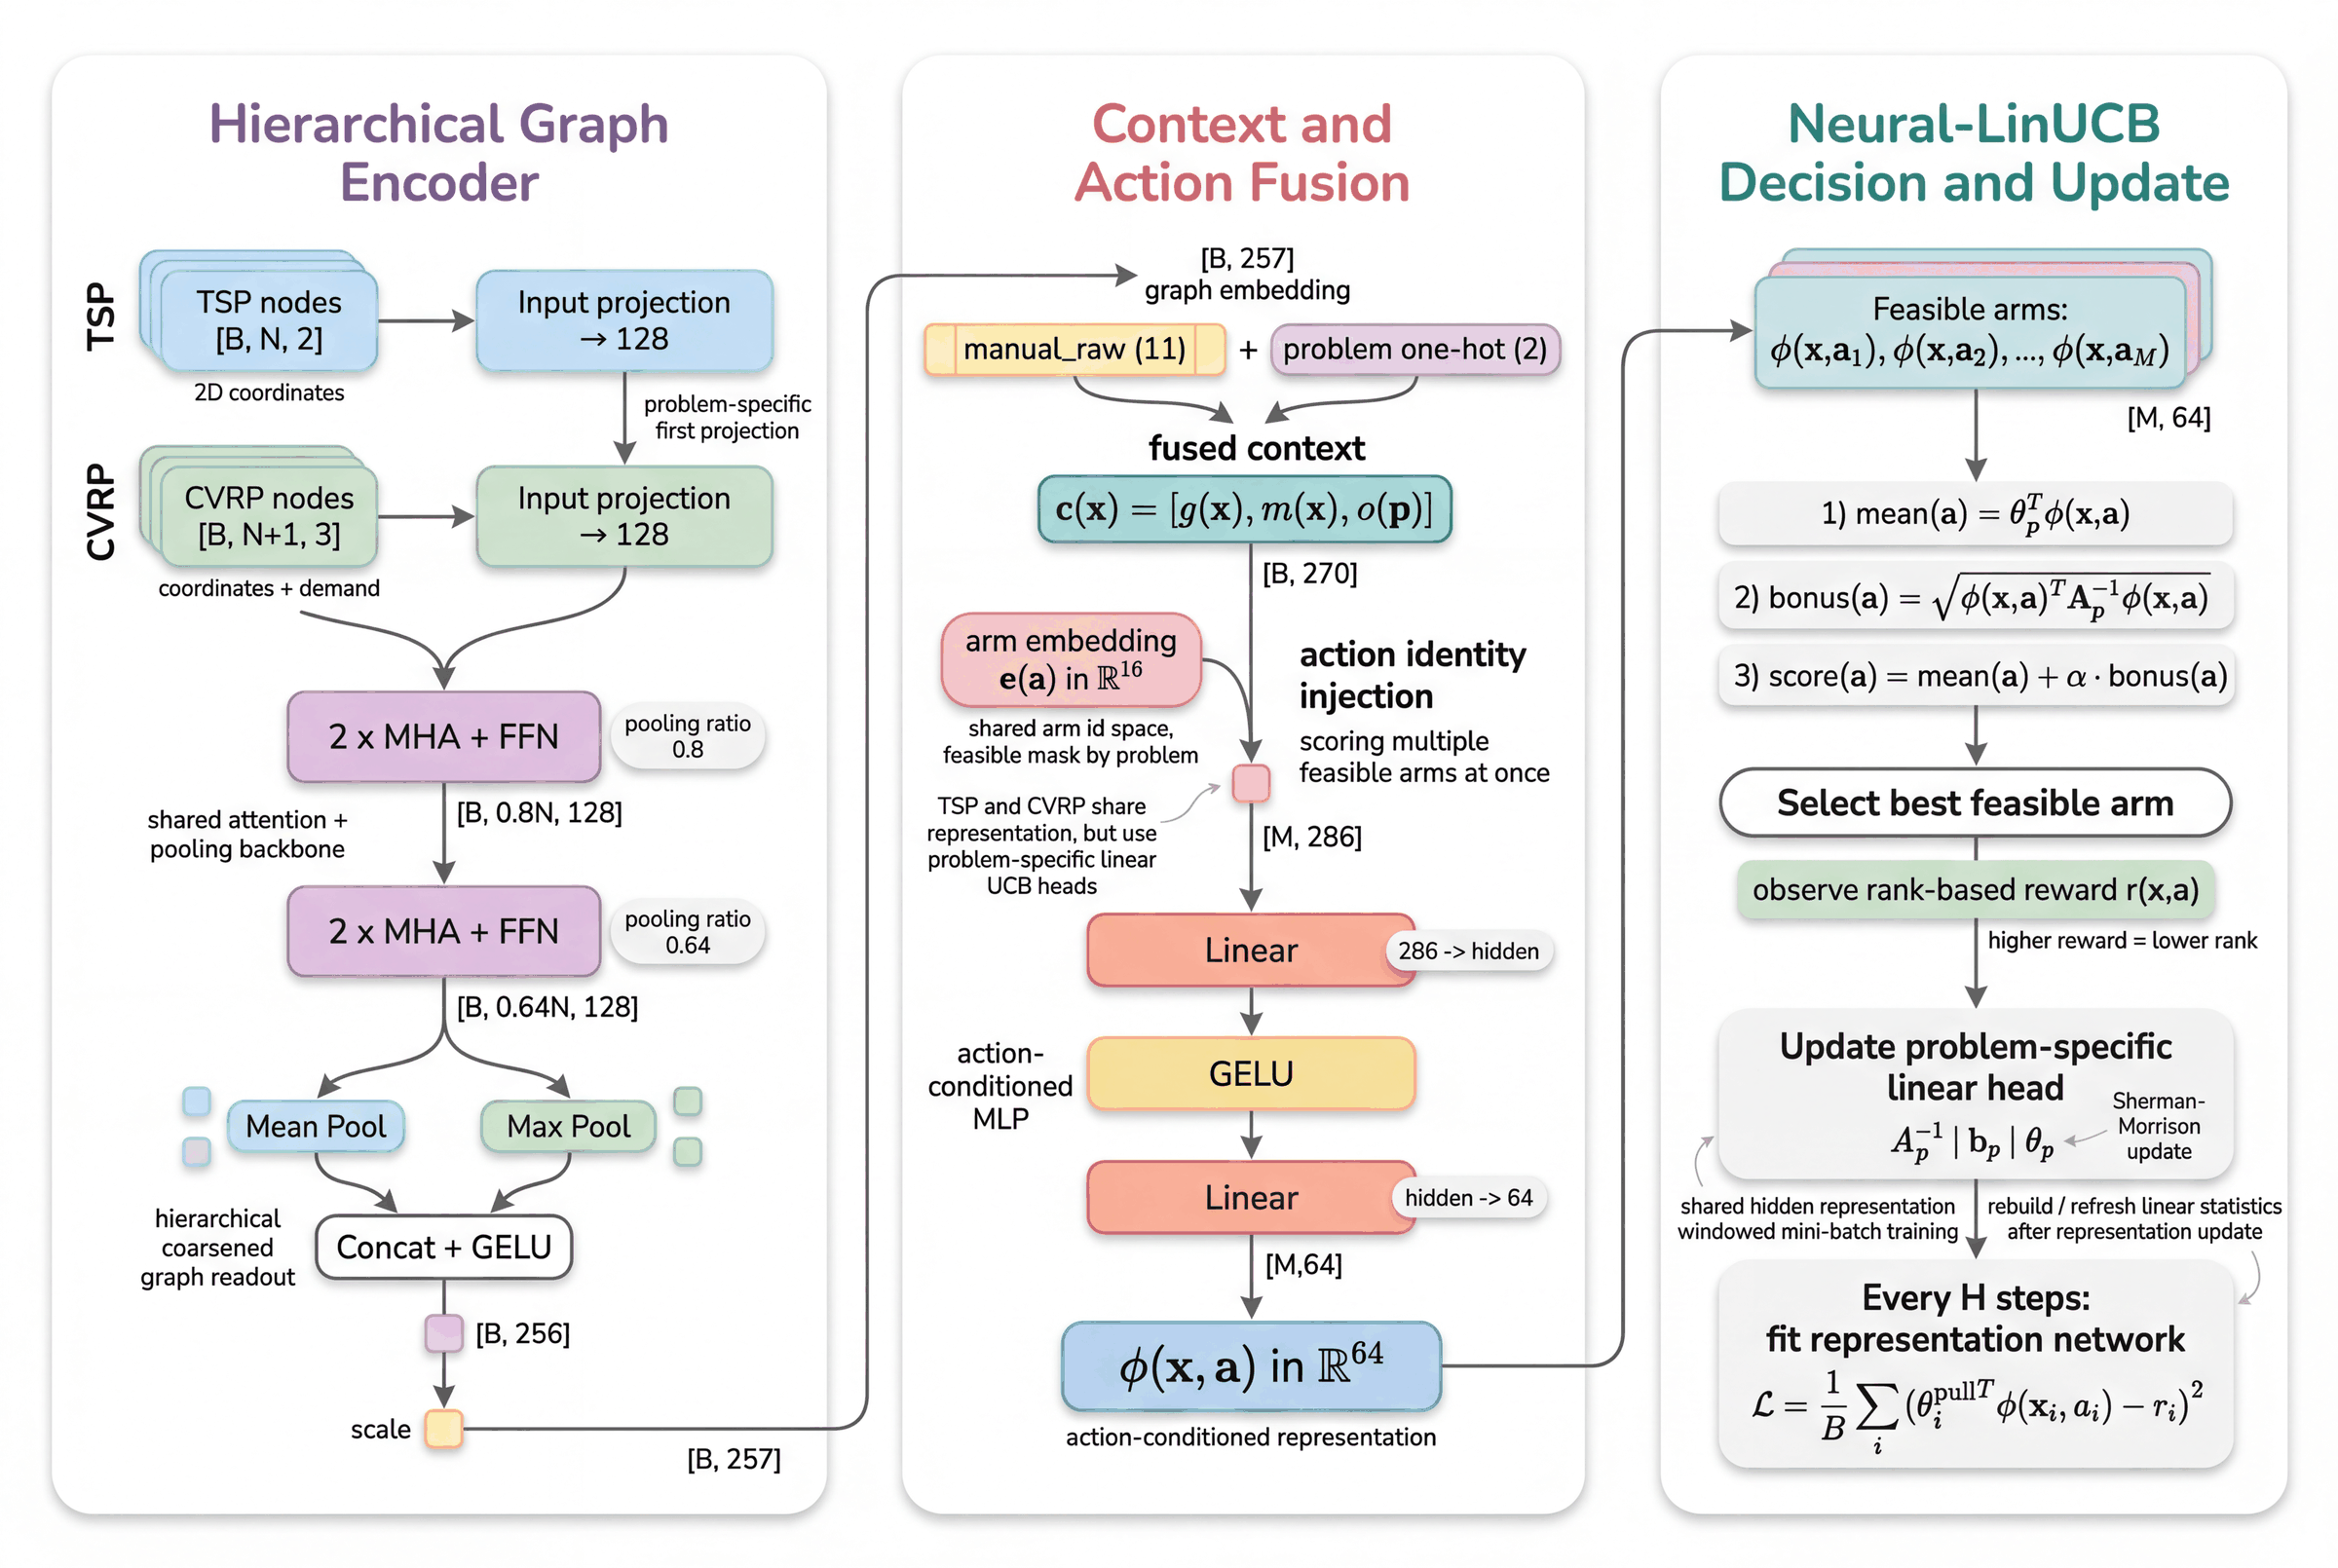
\includegraphics[height=0.8\textheight]{figures/research/figure-07-method-architecture.png.png}
\end{frame}

\begin{frame}[t]{具体实现：实例编码}
  \scriptsize
  \begin{columns}[T,totalwidth=\textwidth]
    \begin{column}{0.54\textwidth}
      \textbf{编码流程与维度}
      \vspace{0.2em}
      \begin{itemize}
        \item TSP 输入为 $\mathtt{[B,n,2]}$，CVRP 输入为 $\mathtt{[B,n+1,3]}$
        \item 问题相关的第一层投影先把节点特征映射到 128 维
        \item 两层 MHA+FFN 与层次池化后，Mean/Max readout 拼接得到 $g(x)\in\mathbb{R}^{256}$
        \item 最终上下文编码为为实例编码256+scale1+手工特征11+问题类型编码2=270维
        \item $c(x)=[g(x),\mathrm{scale},m(x),o(p)]\in\mathbb{R}^{270}$
      \end{itemize}
      \[
        \begin{aligned}
          \mathtt{[B,n,2/3]}
          &\rightarrow
          \mathtt{[B,n+\delta,128]}
          \rightarrow
          \mathtt{[B,0.8n,128]}
          \\
          &\rightarrow
          \mathtt{[B,0.64n,128]}
          \rightarrow
          \mathtt{[B,256]}
          \rightarrow
          \mathtt{[B,257]}
          \rightarrow
          \mathtt{[B,270]}
        \end{aligned}
      \]
    \end{column}
    \begin{column}{0.42\textwidth}
      \centering
      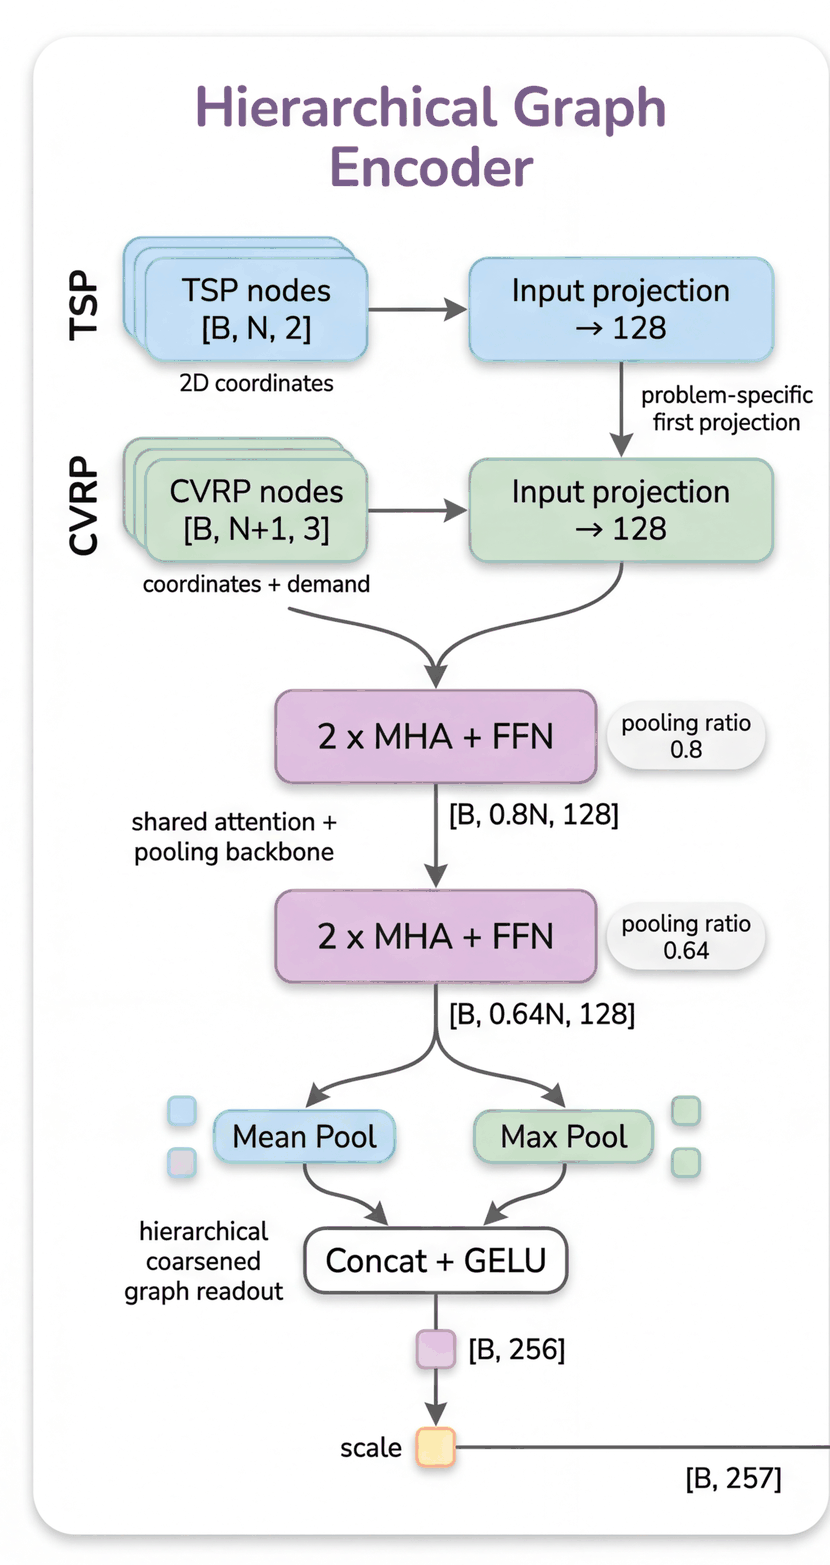
\includegraphics[height=0.76\textheight]{figures/research/slide_crops/method_left.png}
    \end{column}
  \end{columns}
\end{frame}

\begin{frame}[t]{具体实现：动作条件表示}
  \scriptsize
  \begin{columns}[T,totalwidth=\textwidth]
    \begin{column}{0.54\textwidth}
      \textbf{上下文与动作融合}
      \vspace{0.2em}
      \[
        c(x)\in\mathbb{R}^{270},
        \qquad
        e(a)\in\mathbb{R}^{16},
        \qquad
        [c(x),e(a)]\in\mathbb{R}^{286}
      \]
      \[
        \phi(x,a)=f_\psi([c(x),e(a)])\in\mathbb{R}^{64}
      \]
      \begin{itemize}
        \item $e(a)$ 是方法 $a$ 的可学习 arm embedding，$f_\psi$ 是两层 MLP
        \item 同一个实例复制出 $M$ 份上下文，与 $M$ 个候选 arm 的 embedding 分别拼接
        \item 一次前向即可得到 $\phi(x,a_1),\ldots,\phi(x,a_M)$
      \end{itemize}
      \[
        \mathtt{[M,270]}
        +
        \mathtt{[M,16]}
        \rightarrow
        \mathtt{[M,286]}
        \rightarrow
        \mathtt{[M,64]}
      \]
      \begin{itemize}
        \item TSP 与 CVRP 共享表示层，但分别维护自己的 $(A^{-1},b,\theta)$
      \end{itemize}
    \end{column}
    \begin{column}{0.42\textwidth}
      \centering
      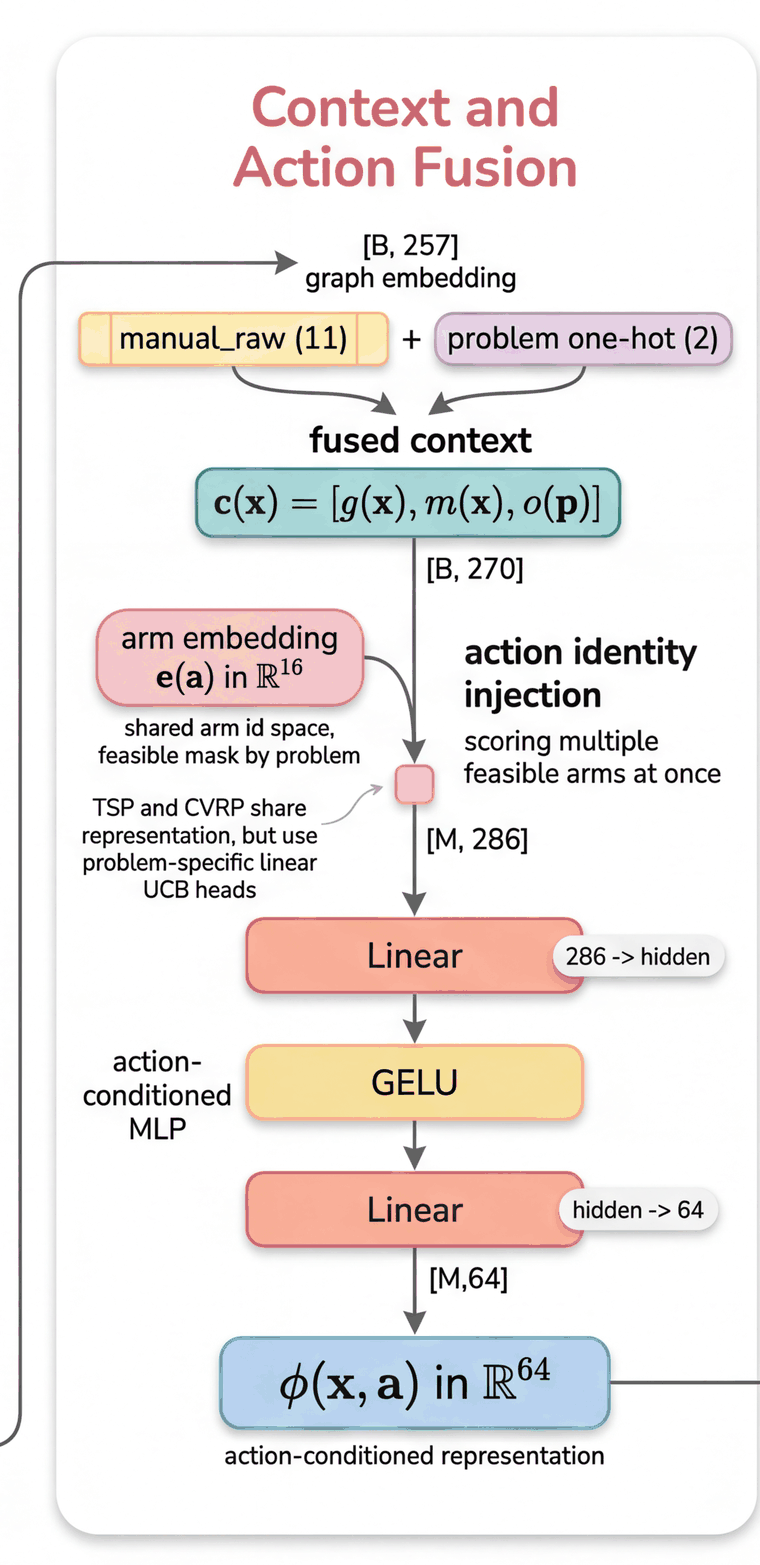
\includegraphics[height=0.76\textheight]{figures/research/slide_crops/method_mid.png}
    \end{column}
  \end{columns}
\end{frame}

\begin{frame}[t]{Neural-LinUCB：动作评分}
  \scriptsize
  \begin{columns}[T,totalwidth=\textwidth]
    \begin{column}{0.58\textwidth}
      \textbf{评分公式}
      \vspace{0.2em}
      \[
        s_t(x_t, a)
        =
        \theta_{p_t,t}^{\top}\phi(x_t, a)
        +
        \alpha \sqrt{\phi(x_t, a)^{\top} A_{p_t,t}^{-1}\phi(x_t, a)}
      \]
      \begin{itemize}
        \item $\phi(x_t,a)\in\mathbb{R}^{64}$：实例与方法的动作条件表示
        \item $\theta_{p_t,t}\in\mathbb{R}^{64}$，$A_{p_t,t}^{-1}\in\mathbb{R}^{64\times64}$，$\alpha$ 为探索强度
        \item 第一项利用，第二项探索，最后在可选 arm 中取 score 最大的方法
      \end{itemize}
    \end{column}
    \begin{column}{0.38\textwidth}
      \centering
      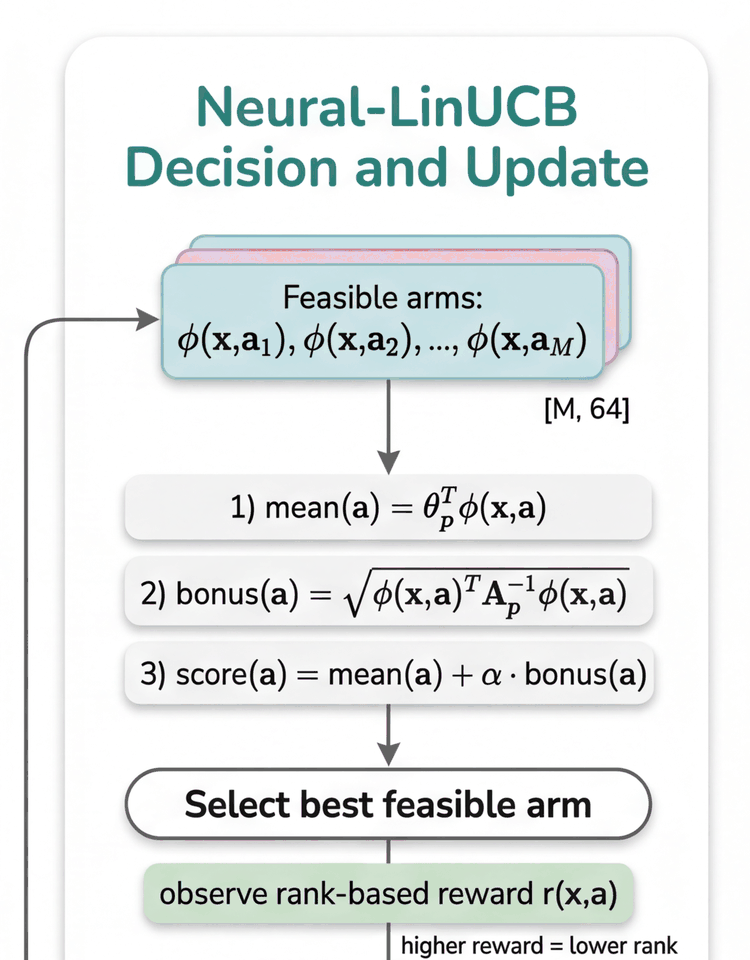
\includegraphics[width=\linewidth]{figures/research/slide_crops/method_score.png}
    \end{column}
  \end{columns}
\end{frame}

\begin{frame}[t]{Neural-LinUCB：线性头在线更新}
  \small
  \begin{columns}[T,totalwidth=\textwidth]
    \begin{column}{0.60\textwidth}
      \textbf{观察反馈后更新线性统计量}
      \vspace{0.2em}
      选中 $a_t$ 并获得 reward $r_t$ 后，更新当前问题对应的线性头：
      \[
        A_{p,t}^{-1}
        \leftarrow
        A_{p,t-1}^{-1}
        -
        \frac{A_{p,t-1}^{-1}\phi_t \phi_t^{\top} A_{p,t-1}^{-1}}
        {1 + \phi_t^{\top} A_{p,t-1}^{-1} \phi_t}
      \]
      \[
        b_{p,t} \leftarrow b_{p,t-1} + r_t \phi_t,
        \qquad
        \theta_{p,t} \leftarrow A_{p,t}^{-1} b_{p,t}
      \]
      \begin{itemize}
        \item $b_{p,t}\in\mathbb{R}^{64}$：reward 加权后的特征累积
        \item $\theta_{p,t}\in\mathbb{R}^{64}$：当前问题的线性 reward 估计
      \end{itemize}
    \end{column}
    \begin{column}{0.36\textwidth}
      \centering
      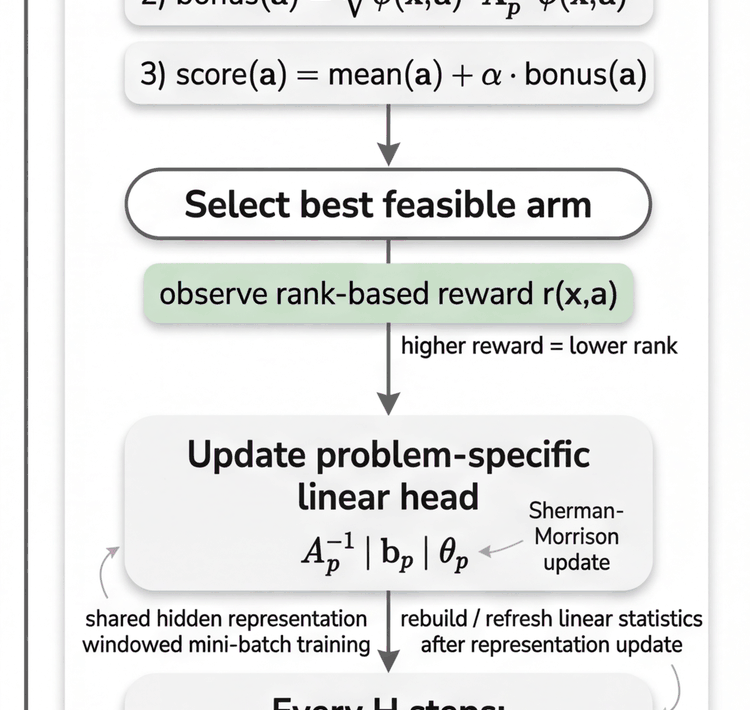
\includegraphics[width=\linewidth]{figures/research/slide_crops/method_update.png}
    \end{column}
  \end{columns}
\end{frame}

\begin{frame}[t]{Neural-LinUCB：表示层周期更新}
  \scriptsize
  \begin{columns}[T,totalwidth=\textwidth]
    \begin{column}{0.58\textwidth}
      \textbf{缓存窗口与训练目标}
      \vspace{0.2em}
      \[
        \mathcal{D}_{\mathrm{rep}}
        =
        \{(x_i,a_i,r_i,\theta_i^{\mathrm{pull}})\}_{i=1}^{B}
      \]
      \[
        \hat{r}_i
        =
        {\theta_i^{\mathrm{pull}}}^{\top}\phi(x_i,a_i),
        \qquad
        \mathcal{L}(\psi)
        =
        \frac{1}{B}
        \sum_{i=1}^{B}
        \left(
          \hat{r}_i-r_i
        \right)^2
      \]
      \begin{itemize}
        \item $r_i$：真实观测到的 reward；$\theta_i^{\mathrm{pull}}$：该样本被选中时缓存的线性头
        \item 不是每一步都重训表示层，而是每隔 $H$ 个 step 做一次窗口化更新
        \item 更新后重建对应问题的 $(A^{-1},b,\theta)$，保证线性头与新特征空间一致
      \end{itemize}
    \end{column}
    \begin{column}{0.38\textwidth}
      \centering
      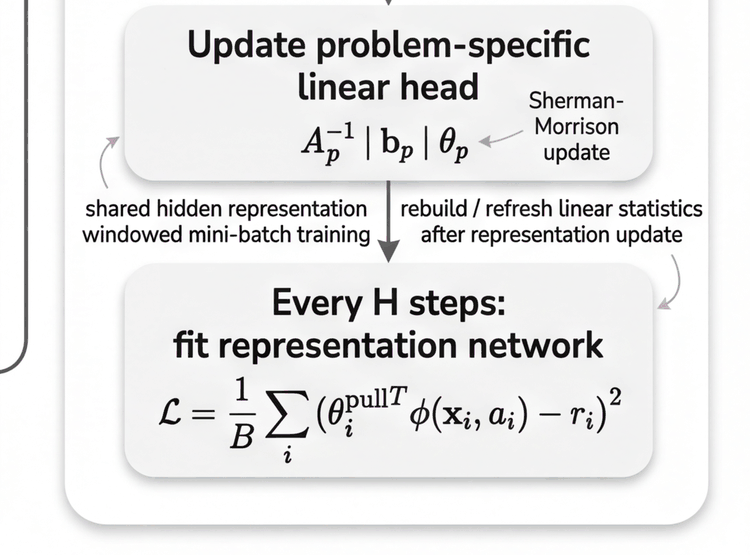
\includegraphics[width=\linewidth]{figures/research/slide_crops/method_repr.png}
    \end{column}
  \end{columns}
\end{frame}

\section{实验}

\begin{frame}{实验设置}
  \scriptsize
  \begin{columns}[T,totalwidth=\textwidth]
    \begin{column}{0.57\textwidth}
      \begin{block}{数据集}
        \textbf{1. 合成混合数据集}
        \begin{itemize}
          \item 训练/验证/测试：TSP 10000 / 1000 / 1000，CVRP 10000 / 1000 / 1000
          \item 规模范围：50--499
          \item 分布：均匀分布 + 高斯混合分布
        \end{itemize}

        \vspace{0.2em}
        \textbf{2. 分布外测试集}
        \begin{itemize}
          \item TSPLIB：49 个实例
          \item CVRPLIB：100 个实例
        \end{itemize}
      \end{block}
    \end{column}
    \begin{column}{0.39\textwidth}
      \begin{block}{评测与对比}
        \textbf{评价指标}
        \begin{itemize}
          \item mean length
          \item top-1 accuracy
        \end{itemize}

        \vspace{0.2em}
        \textbf{比较对象}
        \begin{itemize}
          \item Oracle
          \item SingleBest
          \item 常见的求解方法
        \end{itemize}

        \vspace{0.2em}
        \textbf{关注点}
        \begin{itemize}
          \item 同分布下是否优于固定单方法
          \item 能否泛化到 LIB 基准数据集
        \end{itemize}
      \end{block}
    \end{column}
  \end{columns}
\end{frame}

\section{结果}

\begin{frame}{TSP 结果与分析}
  \tiny
  \centering
  \renewcommand{\arraystretch}{1.02}
  \resizebox{0.98\textwidth}{!}{
  \begin{tabular}{@{}lcccc@{}}
    \toprule
    & \multicolumn{2}{c}{合成混合数据集（1000 实例）} & \multicolumn{2}{c}{TSPLIB（49 实例）} \\
    \cmidrule(lr){2-3}\cmidrule(lr){4-5}
    方法 & mean length $\downarrow$ & top-1 accuracy $\uparrow$ & mean length $\downarrow$ & top-1 accuracy $\uparrow$ \\
    \midrule
    \textbf{Oracle} & 7.8699 & 1.0000 & 8.1422 & 1.0000 \\
    \textbf{Neural-LinUCB} & \textbf{7.9420} & 0.2930 & \textbf{8.2116} & \textbf{0.4490} \\
    \textbf{SingleBest} & 7.9578 & 0.1720 & 8.2334 & 0.1020 \\
    t2t500 & 7.9578 & 0.1720 & 8.2334 & 0.1020 \\
    difusco500 & 7.9580 & 0.1180 & 8.2473 & 0.0612 \\
    t2t & 7.9646 & 0.1110 & 8.2404 & 0.1224 \\
    difusco & 7.9939 & 0.0490 & 8.2645 & 0.0408 \\
    bq & 7.9953 & \textbf{0.3000} & 8.2731 & \textbf{0.4490} \\
    lehd & 8.0365 & 0.1720 & 8.2599 & 0.0816 \\
    elg & 8.0894 & 0.0780 & 8.3842 & 0.1429 \\
    \bottomrule
  \end{tabular}}

  \vspace{0.8em}
  \begin{columns}[T,totalwidth=\textwidth]
    \begin{column}{0.49\textwidth}
      \textbf{合成混合数据集}
      \begin{itemize}
        \item 非 Oracle 最低 mean length：Neural-LinUCB 7.9420
        \item 优于 SingleBest 7.9578
        \item 但 top-1 最优为 \texttt{bq} 0.3000
        \item 排名 reward 与最终 mean length 目标不完全一致
      \end{itemize}
    \end{column}
    \begin{column}{0.49\textwidth}
      \textbf{TSPLIB}
      \begin{itemize}
        \item 非 Oracle 最低 mean length：Neural-LinUCB 8.2116
        \item top-1 accuracy 与 \texttt{bq} 并列最高：0.4490
        \item 说明在 TSP 上有一定分布外泛化能力
      \end{itemize}
    \end{column}
  \end{columns}
\end{frame}

\begin{frame}{CVRP 结果与分析}
  \tiny
  \centering
  \renewcommand{\arraystretch}{1.02}
  \resizebox{0.98\textwidth}{!}{
  \begin{tabular}{@{}lcccc@{}}
    \toprule
    & \multicolumn{2}{c}{合成混合数据集（1000 实例）} & \multicolumn{2}{c}{CVRPLIB（100 实例）} \\
    \cmidrule(lr){2-3}\cmidrule(lr){4-5}
    方法 & mean length $\downarrow$ & top-1 accuracy $\uparrow$ & mean length $\downarrow$ & top-1 accuracy $\uparrow$ \\
    \midrule
    \textbf{Oracle} & 18.1781 & 1.0000 & 68.3098 & 1.0000 \\
    \textbf{Neural-LinUCB} & \textbf{18.2785} & \textbf{0.5770} & 73.7296 & 0.3800 \\
    \textbf{SingleBest} & 18.4167 & 0.4170 & \textbf{68.7926} & \textbf{0.4200} \\
    omni & 18.4167 & 0.4170 & 69.0533 & 0.3100 \\
    bq & 18.6225 & 0.2050 & 72.4496 & 0.1500 \\
    lehd & 18.6556 & 0.2520 & 77.2945 & 0.1100 \\
    elg & 18.6643 & 0.0770 & \textbf{68.7926} & \textbf{0.4200} \\
    mvmoe & 19.6954 & 0.0490 & 76.1748 & 0.0100 \\
    \bottomrule
  \end{tabular}}

  \vspace{0.8em}
  \begin{columns}[T,totalwidth=\textwidth]
    \begin{column}{0.49\textwidth}
      \textbf{合成混合数据集}
      \begin{itemize}
        \item mean length 与 top-1 accuracy 都优于固定单方法
        \item Neural-LinUCB：18.2785 / 0.5770
        \item 说明实例条件化选择在同分布下有效
      \end{itemize}
    \end{column}
    \begin{column}{0.49\textwidth}
      \textbf{CVRPLIB}
      \begin{itemize}
        \item Neural-LinUCB：73.7296 / 0.3800
        \item SingleBest 与 \texttt{elg}：68.7926 / 0.4200
        \item 当前方法在 CVRP 上的分布外泛化仍不足
      \end{itemize}
    \end{column}
  \end{columns}
\end{frame}

\begin{frame}{训练损失曲线与结果解释}
  \scriptsize
  \begin{columns}[T,totalwidth=\textwidth]
    \begin{column}{0.38\textwidth}
      \textbf{观察}
      \begin{itemize}
        \item loss 持续下降，训练过程数值稳定
        \item step 6000 左右进入平台期，后续下降幅度很小
      \end{itemize}

      \vspace{0.4em}
      \textbf{解释}
      \begin{itemize}
        \item 当前 reward 采用实例内排名
        \item 排名丢失了方法之间的绝对长度差距信息
        \item 因此 loss 下降不一定同步带来更优的 mean length
      \end{itemize}
    \end{column}
    \begin{column}{0.58\textwidth}
      \centering
      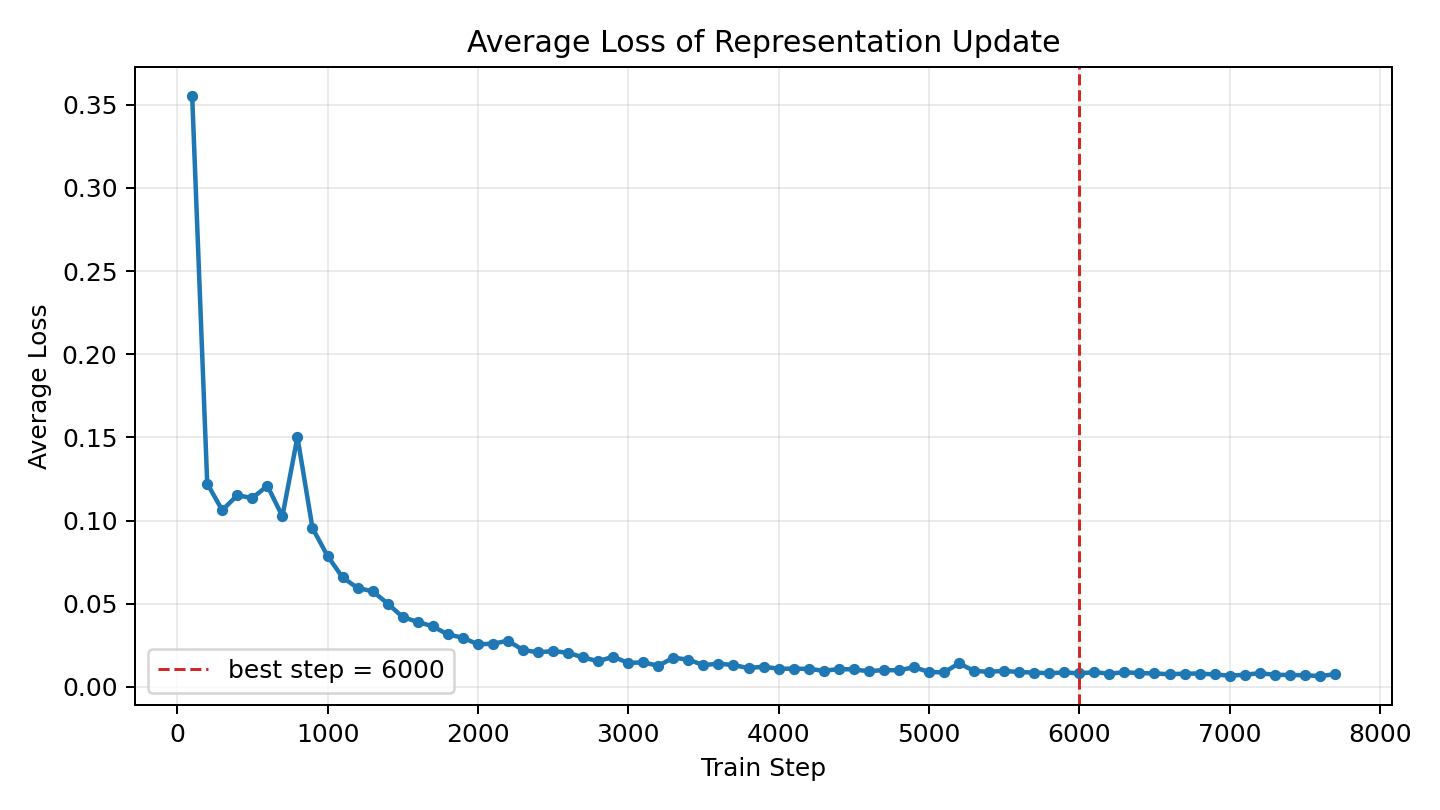
\includegraphics[width=\linewidth]{figures/research/figure-06-training-loss.png}
    \end{column}
  \end{columns}
\end{frame}

\begin{frame}{负结果分析：不同决策粒度的比较}
  \scriptsize
  \begin{block}{研究路径比较}
    \centering
    \renewcommand{\arraystretch}{1.15}
    \begin{tabular}{p{0.28\textwidth}p{0.56\textwidth}}
      \toprule
      研究路径 & 决策粒度 \\
      \midrule
      双门控强化学习 & 初始化一次 + 迭代器一次 \\
      步级算子选择 & 初始化一次 + 每步选算子 \\
      初始化选择 & 初始化一次 \\
      \bottomrule
    \end{tabular}
  \end{block}

  \vspace{0.4em}

  \begin{block}{结论}
    \begin{itemize}
      \item 在确定当前框架之前，曾尝试过更细粒度的两类决策建模方式。
      \item 前两类设定都出现了明显的策略坍缩，训练后期会退化为少数固定选择。
      \item 因此最终将问题收缩为“只在初始化阶段做一次选择”的上下文老虎机。
    \end{itemize}
  \end{block}
\end{frame}

\begin{frame}{负结果：更细粒度控制容易坍缩}
  \centering
  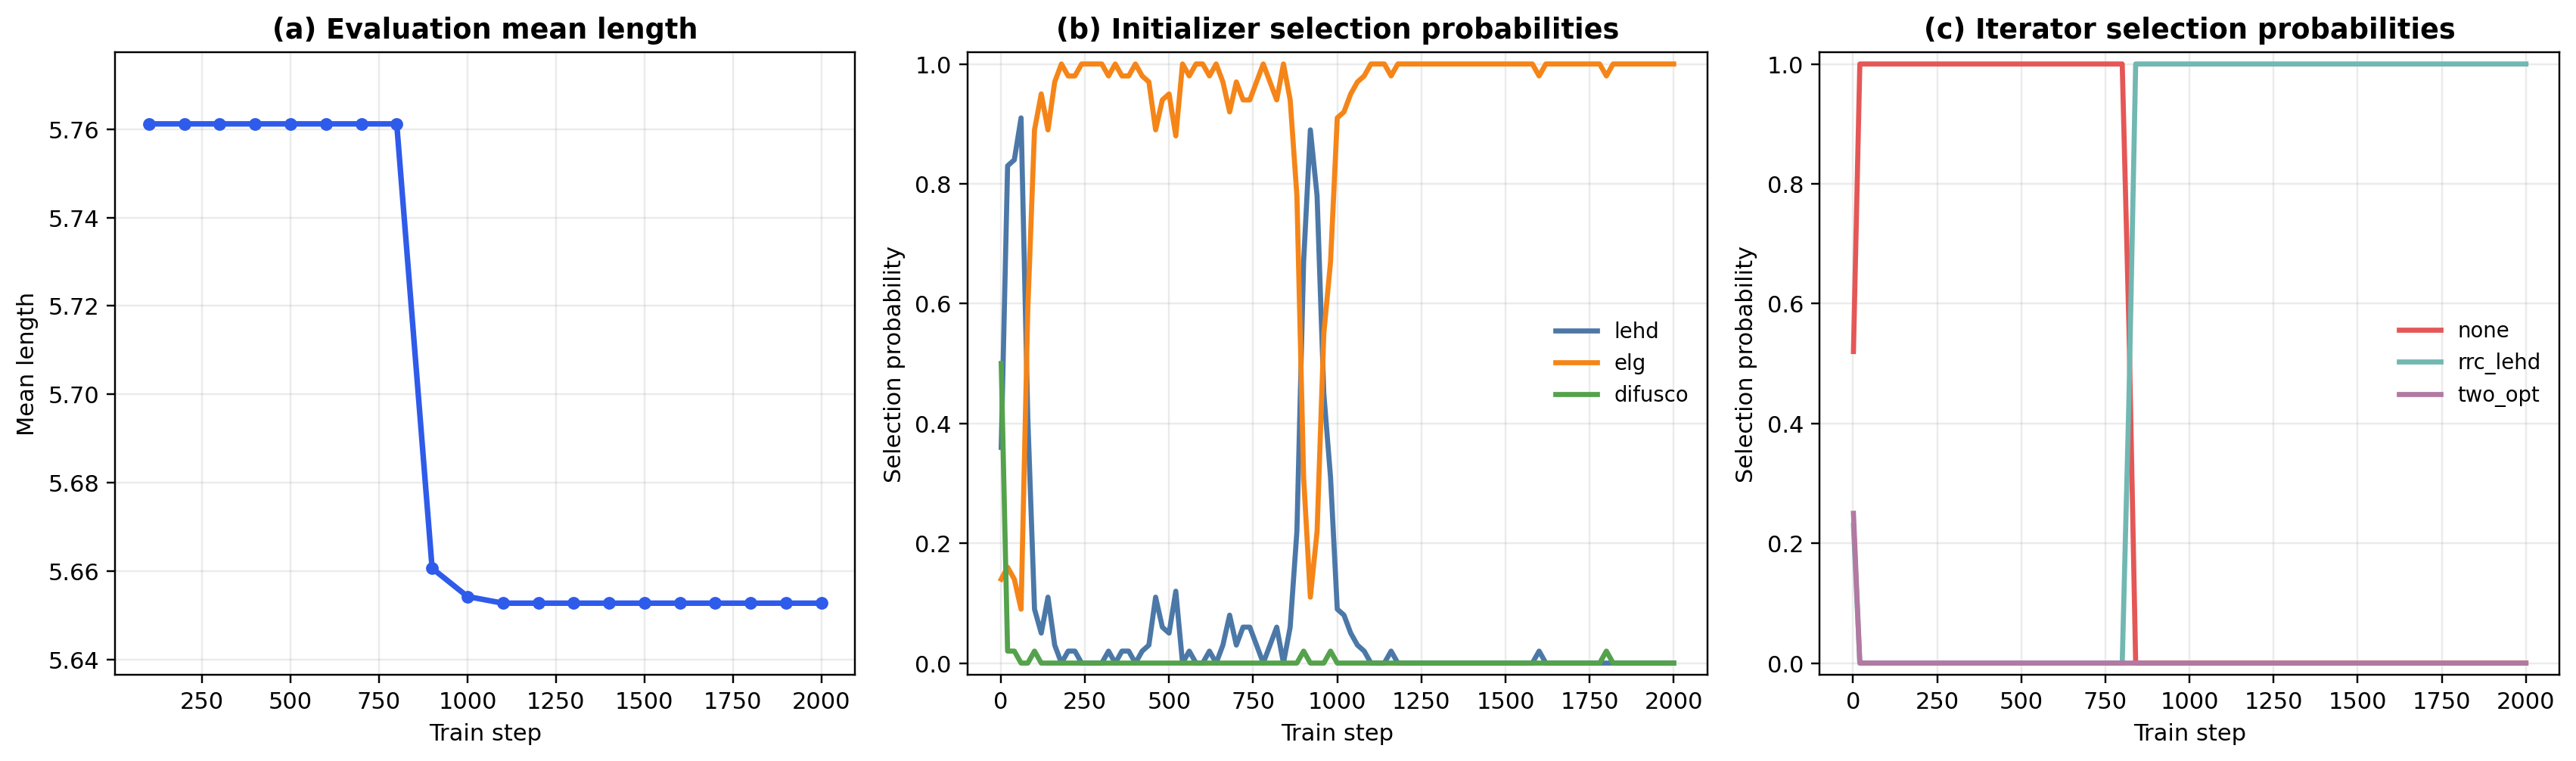
\includegraphics[width=\textwidth]{figures/research/figure-05-two-gate-collapse-triptych.png}

  \vspace{0.4em}
  \scriptsize
  \begin{itemize}
    \item 双门控强化学习中，初始化选择最终固定到 \texttt{elg}，迭代阶段则固定到 \texttt{rrc\_lehd\_10}。
    \item 评测 mean length 只在切换附近出现一次跃迁，随后基本进入平台期。
    \item 这说明更细粒度的控制在当前动作设计和奖励条件下更容易退化为确定性的单一策略。
  \end{itemize}
\end{frame}

\section{总结}

\begin{frame}{总结与展望}
  \scriptsize
  \begin{block}{结论}
    \begin{itemize}
      \item 使用上下文老虎机解决初始化方法选择
      \item 共享表示层 + 问题特定线性头
      \item 分布内有效，分布外泛化仍弱
    \end{itemize}
  \end{block}

  \vspace{0.5em}

  \begin{block}{后续工作}
    \begin{itemize}
      \item reward 重设：从实例内排名转向 gap、relative improvement 等
      \item 扩展到更多组合优化问题
      \item 两阶段框架：初始化选择 + 迭代阶段方法调度
      \item 分布外泛化：TSPLIB / CVRPLIB 上的 domain shift 适配
      \item 系统消融实验：reward、window、arm embedding、表示维度
      \item 与更多 selector / bandit / supervised baseline 对比
    \end{itemize}
  \end{block}
\end{frame}

\begin{frame}
  \centering
  \Huge 谢谢！
\end{frame}

\end{document}
